\documentclass[a4paper,12pt]{article}
\usepackage{graphicx}    % needed for including graphics e.g. EPS, PS
\topmargin -1.5cm        % 
\oddsidemargin -0.04cm   % 
\evensidemargin -0.04cm  % same as oddsidemargin but for left-hand pages
\textwidth 16.2cm
\textheight 24.80cm 

%\usepackage[top=1cm,right=3cm,nohead,nofoot]{geometry}

% Title Page
\title{{\bf Assignment Learning from Data}}
\author{0501050 \hspace{42pt} Ting-Shuo Yo\\
        0501247 \hspace{16pt} Shriprakash Sinha}
\date{}
\begin{document}
\maketitle


%%%%%%%%%%%%%%%%%%%%%%%%%%%%%%%%%%%%%%%%%%%%%%%%%%%%
% Section 1
%%%%%%%%%%%%%%%%%%%%%%%%%%%%%%%%%%%%%%%%%%%%%%%%%%%%
\section{Introduction}
Given a dataset of size $n=200$, a classification model supposed to be constructed for the underlying population. The dataset contains numerical independent variables ${\bf X}=\{X_1,X_2,X_3\}$ and binary class label $Y$, and not all independent variables are predictive for $Y$.

To learn a classifier with minimal error rate and to provide an proper estimate for the error rate, a systematic analysis process is performed.  The rationale of this analysis process is discussed in section 2, and the corresponding results of each step are summarised in section 3.  In section 4, we give the best learned model and a few concluding remarks.

%%%%%%%%%%%%%%%%%%%%%%%%%%%%%%%%%%%%%%%%%%%%%%%%%%%%
% Section 2
%%%%%%%%%%%%%%%%%%%%%%%%%%%%%%%%%%%%%%%%%%%%%%%%%%%%
\section{Methods}
Following is the analysis procedure used for this assignment:

\begin{enumerate}
\item {\bf Explore the given dataset}\\
First step of the analysis is to explore the basic properties of the given dataset.  Since it is hinted that some independent variables are not predictive at all, to find a proper formula for models to fit may be a good start.  In this step, we look at the correlation coefficients among variables and perform a few runs of step-wise logistic regression.  Afterward, a few candidate formulas are used for later steps.

\item {\bf Test several classification algorithms} \\ 
  Following classification algorithms are tested: logistic regression, linear/quadratic discriminant analysis, neural networks, $k$-nearest neighbour, and support vector machines.  Each classifier is tested with a few combination of parameters, and the most proper parameter sets are decided upon the resulting error rates of the re sampling tests.

  With the "best" parameter sets, all algorithms are compared together by their error rates on the same re sampling datasets.  A few candidate algorithm-parameter combination are used for the next step.

\item {\bf Bootstrap aggregating with adaptive resampling}\\
For all survival candidates in previous step, bagging and boosting techniques are applied to improve their performance (i.e., to lower the error rates).  {\bf The final decision will be made upon the final performance measure.}

\end{enumerate}


%%%%%%%%%%%%%%%%%%%%%%%%%%%%%%%%%%%%%%%%%%%%%%%%%%%%
% Section 3
%%%%%%%%%%%%%%%%%%%%%%%%%%%%%%%%%%%%%%%%%%%%%%%%%%%%
\section{Results}
\subsection*{\bf Candidate formulas}
The correlation matrix for $x.1, x.2, x.3$, and $y$ shows that $x.3$ has little correlation to other variables ($<$ 0.1). Meanwhile, the step-wise logistic regression (use AIC for model selection) with 20-fold cross validation also shows a preference to the formula: $y = x.1 + x.2^2$ (17 out of 20).  Therefore, two formulas, i.e., linear and $y = x.1 + x.2^2$ are considered for following tests, and are referred as f1 and f2.


\subsection*{\bf Candidate classifiers and parameter sets}
The error rates are used as the performance measure, and calculated based on in-sample, cross-validation (2-, 5-, 10-, 20-, 50-, 100-fold, and leave-one-out) and bootstrapping (100 resampling).  The best parameter set for each classifier is described below.

\begin{enumerate}
\item {\bf logistic regression}\\
For in-sample and cross-validation with 2 $\sim$ 100 folds, models with f1 perform slightly better than ones with f2, as well as the estimation with bootstrapping.  However, for leave-one-out cross-validation, f1 and f2 are with similar error rate.  Hence, both models are considered for next step, and are referred as LR1 and LR2.

\item {\bf linear/quadratic discriminant analysis}\\
For all error rate estimates, f2 is slightly better. Also, LDA performs slightly better than QDA.  Here, we decide to use both LDA and QDA with f2 for next step.

\item {\bf $k$-nearest neighbour}\\
No formula is applied to this non-parametric classifier.  The value of $k$ is tests from 1 to 10, and the best performance can be found around $k$ = 5 $\sim$ 10.  This does not include the in-sample test, because the 1NN will always be $100\%$ correct in this case.  Therefore, $k$ = 5 is used for later step.

\item {\bf neural network}\\
An implementation of one-hidden-layer neural network is tested with formula = $\{f1,f2\}$, size of hidden layer = $\{2,4,6,8,10\}$, decay = $\{0.01, 0.001, 0.0001\}$, and activation functions = $\{softmax, entropy\}$ ($softmax$ is tested only for f1 due to technical reasons).  After comparing the estimated error rates, $\{size = 4, decay = 0.01, entropy\}$ for both f1 and f2 are selected.

\item {\bf support vector machine}\\
A SVM implementation in the package {\bf e1071} is used for the test.  Kernels can be chosen from $\{linear, polynomial, radial-basis, sigmoid\}$, and $linear$ kernel is selected along with formula f1.

\end{enumerate}
A summary of the tests is shown in table \ref{compall}.  Since the $5$-NN tends to have higher error, it will not be considered in the next step.

\begin{table}
\begin{center}
\caption[summary comparison]{Summary of the mean error rates for each classifier}
\label{compall}
\begin{tabular}{ccccccccc}
\hline
              & LR1   & LR2   & LDA2  & QDA2  & 5-NN  & NNET1 & NNET2 & SVM \\
\hline
in-sample     & 0.250 & 0.245 & 0.245 & 0.275 & 0.200 & 0.140 & 0.116 & 0.240 \\
10-fold CV    & 0.250 & 0.255 & 0.250 & 0.270 & 0.265 & 0.290 & 0.160 & 0.270 \\
leave-one-out & 0.260 & 0.260 & 0.255 & 0.275 & 0.290 & 0.240 & 0.160 & 0.260 \\
100 bootstrap & 0.265 & 0.259 & 0.262 & 0.276 & 0.311 & 0.265 & 0.265 & 0.263 \\
\hline
\end{tabular}
\end{center}
\end{table}


\subsection*{\bf Bagging and Boosting}
All classifiers in table \ref{compall} except $5$-NN are applied to bootstrap aggregating of 10, 50, and 100 models trained by resampling.  The error rate of ensemble predictions on the whole dataset are considered.  In our experiments, each classifier gains 0.01 $\sim$ 0.02 in their performance, and only LR1, NNET1, and NNET2 keep improving as the number of bagging models increases.  Therefore, these three classifiers are further combined with an adaptive-resampling scheme, i.e., arc-x4.

Combing with arc-x4, the performance of LR1 does not improve at all, while NNET1 and NNET2 have their error rate improved to 0.080 and 0.145 for just 10 resampling models.  Since NNET1 wins out eventually, we further test how much can its performance be improved with increasing resampling process.

Table \ref{perftab} shows the results of the experiment.  As we can see from the table, the best performance can be found at 500 ensemble models for an error rate of 0.01395.  

%\begin{figure}
%\centering
%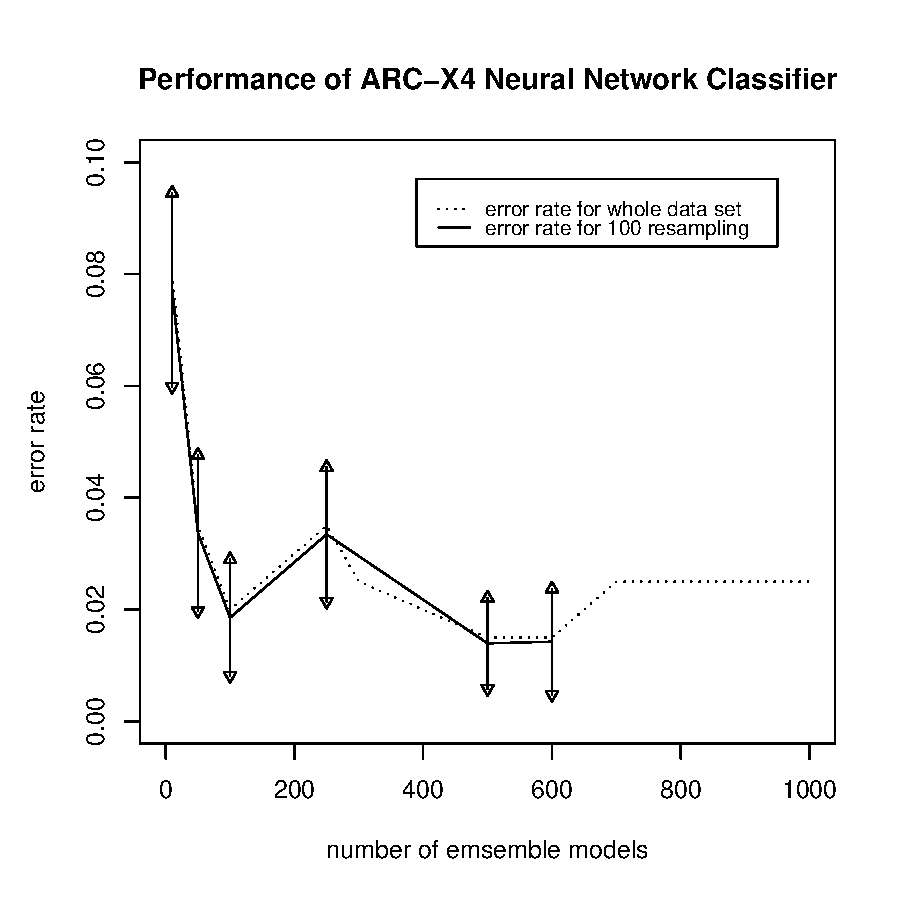
\includegraphics[scale=0.8]{perf.ps}
%\caption{Caption goes here}
%\label{performance}
%\end{figure}

\begin{table}
\begin{center}
\caption[arc-nnet]{Error rates of arc-x4 neural network classifier.}
\label{perftab}
\begin{tabular}{cccccccc}
\hline
         & 10    & 50    & 100   & 250   & 500   & 600   & 1000 \\
\hline
All Data & 0.08000 & 0.03500 & 0.02000 & 0.03500 & 0.01500 & 0.01500 & 0.02500 \\
100 resampling & & & & & & & \\
Mean & 0.07720 & 0.03370 & 0.01855 & 0.03345 & 0.01395 & 0.01425 & \\
Std  & 0.01731 & 0.01392 & 0.01038 & 0.01199 & 0.00811 & 0.00946 & \\
\hline
\end{tabular}
\end{center}
\end{table}


%%%%%%%%%%%%%%%%%%%%%%%%%%%%%%%%%%%%%%%%%%%%%%%%%%%%
% Section 4
%%%%%%%%%%%%%%%%%%%%%%%%%%%%%%%%%%%%%%%%%%%%%%%%%%%%
\section{Concluding remarks}
By performing student's t-test (one-tail) among the best three candidates, i.e, 100, 500, and 600 models, we found that 500-model is not significantly better (p=0.05) than 600-model, but both 500 and 600 are significantly better than 100-model ensemble.  Considering the 100-resampling will be preferable to the significance ($p$ = 0.001), we made another 10-resampling test, and the 500-model is not better than 100-model anymore.

Next, we need to choose from 500-model and 600-model.  Taking the computation effort into consideration, we concluded that 500-model ensemble for arc-x4 neural network is the best classifier we can find.  And the 95\% confidence interval for its estimate error rate is 0.01233 $\sim$ 0.01557.  However, if the cost of computation is weighted more, the 100-model ensemble for arc-x4 neural network is also an acceptable alternative, with a estimate error rate (95\% confidence interval) of  
0.01647 $\sim$ 0.02063.

Our $pred.class(x)$ will by default use 500-model ensemble, and an alternative with less computational cost can be test by specifying the number of models, e.g., $pred.class(x, 100)$.

\end{document}          
